\documentclass[onlytextwidth, aspectratio=169]{beamer}
\usepackage[utf8]{inputenc}
\usepackage{microtype}
\usepackage{amsmath}
\usepackage{amssymb}
\usepackage[nomessages]{fp} %\FPeval{\var-name}{2*sin(pi/6)}
\usepackage{siunitx} %units in math. eg 20\milli\meter
\usepackage{yhmath} % for arcs, overparenth command
\usepackage{tikz} %graphics
\usetikzlibrary{quotes, angles, arrows, arrows.meta}
%\usepackage{graphicx} already loaded by beamer class
%consider setting \graphicspath{{images/}}
%\parskip ?? to avoid paragraph indent
\usepackage{multicol} %may not need this package, just columns environment
\usepackage{venndiagram}

\subtitle[BECA]{Bronx Early College Academy}
\author[Huson]{Christopher J. Huson PhD}

\setbeamertemplate{headline}{\vskip2mm 
  \, BECA / \insertshortauthor \, / \inserttitle
  \hfill 
  \insertsection
  }

%Tick mark commands
\newcommand\ticks{}
  \def\ticks{{Bar[scale=2]}-{Bar[scale=2]}}
\newcommand\paraticks{}
  \def\paraticks{{Straight Barb[reversed, scale=2]}-{Straight Barb[scale=2]}}

\title{Geometry Unit 7: Congruence transformations}
\date{17 January 2023 - 3 February 2023}

\begin{document}
\frame{\titlepage}
\section[Outline]{}
\frame{\tableofcontents}

\section{7.1 Translation \hfill 17 January \,}
\begin{frame}{Learning Target: I can slide a figure}
  {HSG.CO.A.5 Congruence transformations \hfill \alert{7.1 Tuesday 17 January}}
  \begin{columns}
    \column{0.6\textwidth}
    Do Now
    \begin{enumerate}
      \item Review your Jumprope grades
      \item Find the rise and run of the line segment $\overline{AB}$.
    \end{enumerate}
    Lesson: Translation, classwork practice \\
    Homework: Deltamath practice
    \column{0.4\textwidth}
    \begin{flushright}
      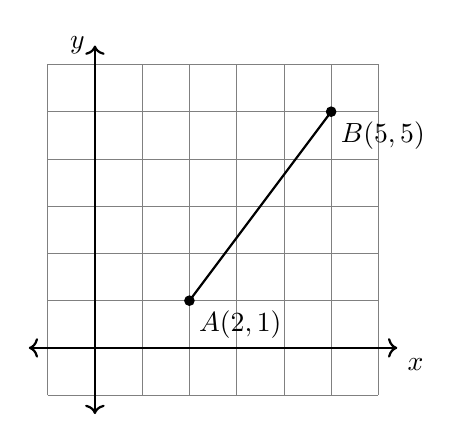
\begin{tikzpicture}[scale=0.6]
        \draw[help lines] (-1,-1) grid (6,6);
        \draw[thick, <->] (-1.4,0) -- (6.4,0) node [below right] {$x$};
        \draw[thick, <->] (0,-1.4)--(0,6.4) node [left] {$y$};
        \draw[thick,domain=2:5] plot (\x, 1.333*\x-1.667);
        \draw [fill] (2,1) circle [radius=0.1] node[below right] {$A(2,1)$};
        \draw [fill] (5,5) circle [radius=0.1] node[below right] {$B(5,5)$};
      \end{tikzpicture}
    \end{flushright}
  \end{columns}
\end{frame}

\begin{frame}{Translation}
    \begin{columns}
      \column{0.6\textwidth}
      Rise is plus 4, run is plus 3. \\
      $$A(2,1) \rightarrow B(5,5)$$
      \begin{description}
        \item[Translate] Move a figure horizontally and vertically (slide)
        \item[Vector] A quantity with both magnitude and direction 
        $$\overrightarrow{AB}=(3,4)$$
      \end{description}
      \column{0.4\textwidth}
      \begin{flushright}
        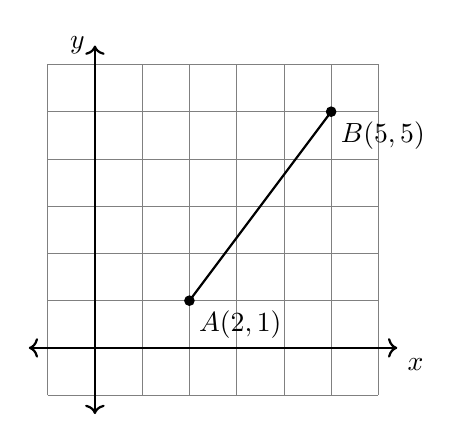
\begin{tikzpicture}[scale=0.6]
          \draw[help lines] (-1,-1) grid (6,6);
          \draw[thick, <->] (-1.4,0) -- (6.4,0) node [below right] {$x$};
          \draw[thick, <->] (0,-1.4)--(0,6.4) node [left] {$y$};
          \draw[thick,domain=2:5] plot (\x, 1.333*\x-1.667);
          \draw [fill] (2,1) circle [radius=0.1] node[below right] {$A(2,1)$};
          \draw [fill] (5,5) circle [radius=0.1] node[below right] {$B(5,5)$};
        \end{tikzpicture}
      \end{flushright}
    \end{columns}
  \end{frame}

\begin{frame}{Example: Translate point $A$ up two units and right four units}
    \begin{columns}
    \column{0.6\textwidth}
        Notation for translation: \\
        $$\overrightarrow{AA'}=(+4,+2)$$
        $$A(2,1) \rightarrow A'(2+4,1+2)$$
        $$T_{+4,+2}$$
        \begin{description}
            \item[Pre-image] The original figure
            \item[Image] The result of a transformation
            \item[Prime] The prime symbol is used to denote the image ($A'$)
          \end{description}
    \column{0.4\textwidth}
    \begin{flushright}
    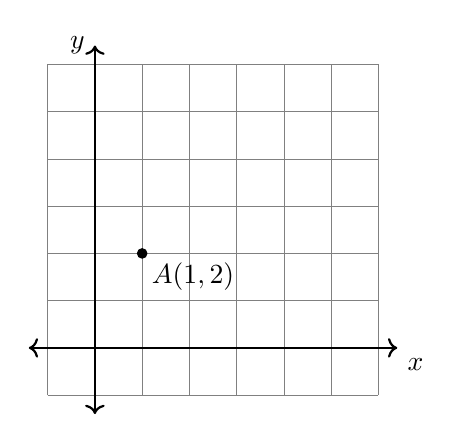
\begin{tikzpicture}[scale=0.6]
        \draw[help lines] (-1,-1) grid (6,6);
        \draw[thick, <->] (-1.4,0) -- (6.4,0) node [below right] {$x$};
        \draw[thick, <->] (0,-1.4)--(0,6.4) node [left] {$y$};
        \draw [fill] (1,2) circle [radius=0.1] node[below right] {$A(1,2)$};
    \end{tikzpicture}
    \end{flushright}
\end{columns}
\end{frame}

\begin{frame}{Translate $\triangle ABC$ right one unit and up three units $T_{+1,+3}$}
    \begin{columns}
    \column{0.6\textwidth}
        $$(x,y) \rightarrow (x+1,y+3)$$
        $$A(1,1) \rightarrow$$
        $$B(2,1) \rightarrow$$
        $$C(4,1) \rightarrow$$

        \begin{description}
            \item[Rigid motion] Move without changing the shape or size (isometry)
            \item[Congruent] Figures with the same size and shape
            \item[Invariant] Does not change (lengths, angles, area, perimeter)
          \end{description}
    \column{0.4\textwidth}
    \begin{flushright}
    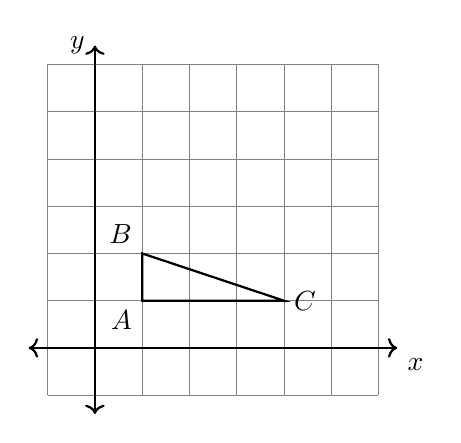
\begin{tikzpicture}[scale=0.6]
        \draw[help lines] (-1,-1) grid (6,6);
        \draw[thick, <->] (-1.4,0) -- (6.4,0) node [below right] {$x$};
        \draw[thick, <->] (0,-1.4)--(0,6.4) node [left] {$y$};
        \draw[thick] (1,2)node[above left]{$B$} --(1,1)node[below left]{$A$} --
            (4,1) node [right] {$C$} --cycle;
    \end{tikzpicture}
    \end{flushright}
\end{columns}
\end{frame}

\end{document}